\vspace{-0.3cm}
\section{晶圆级 GEMV}\label{sec:gemv}
\vspace{-0.2cm}

本节介绍 \gemv：一种面向 PLMR 设备的可扩展 GEMV 算法。

\subsection{分布式 GEMV 的 PLMR 符合性}

\begin{figure}[t!]
    \centering
    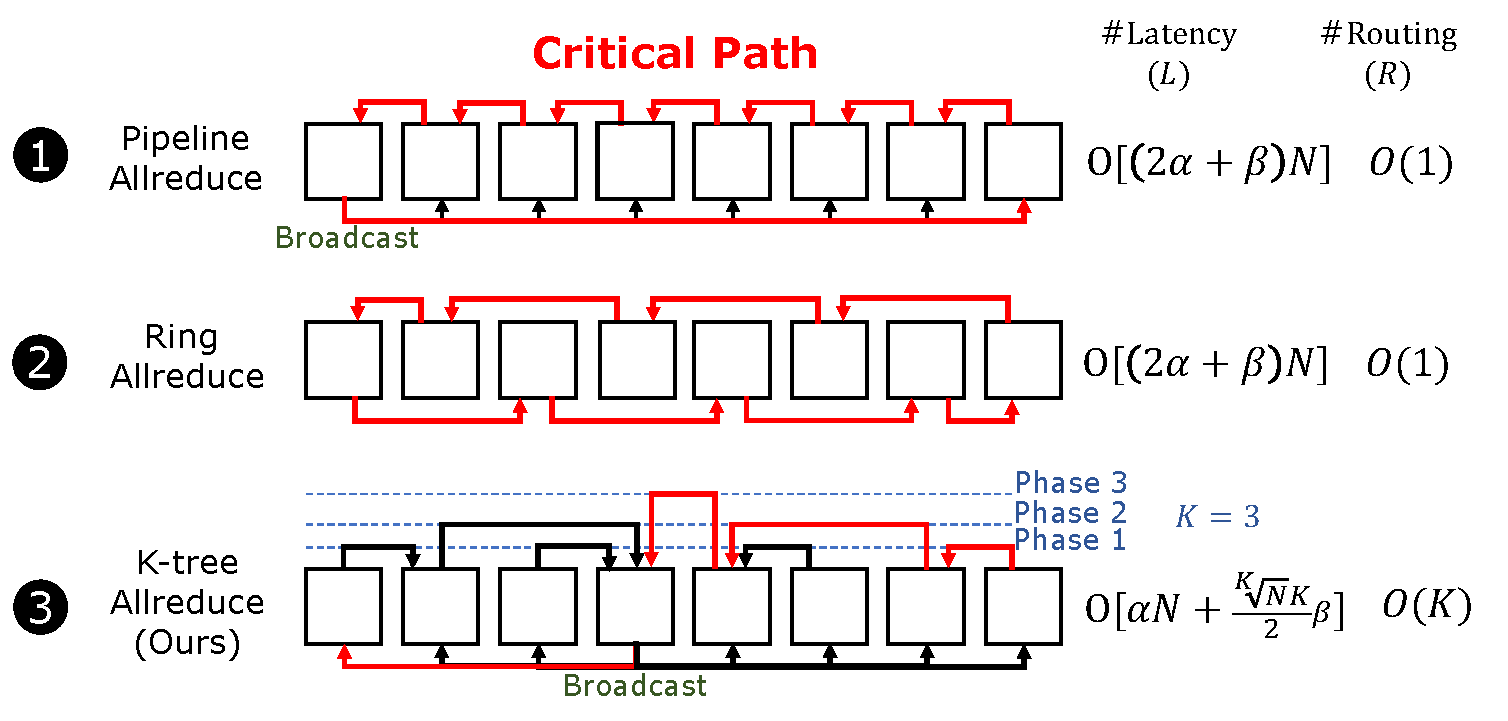
\includegraphics[width=1\linewidth]{imgs/reduce-algo.pdf}
    \caption{分布式 GEMV 的 PLMR 符合性}
    \label{fig:gemv-plmr-compliance}
\end{figure}

分布式 GEMV 的完成时间主要由两部分决定：首先，每个核心执行逐元素计算，生成局部部分和；随后，allreduce 聚合所有选中核心的部分结果，并把聚合结果发回所有核心，以便继续执行 GEMV。与 GEMM 的分析类似，我们也为晶圆级 GEMV 定义以下指标：
（i）\emph{单核路由路径数}：每个核心使用的路由路径数量；路径越少，越符合 R 属性。
（ii）\emph{关键路径延迟}：整个 allreduce 通信的最大延迟，主要由从最远核心发送部分和，到该核心收到聚合和之间的时间决定。

下面分析现有分布式 GEMV 方法，并说明 \gemv 如何满足这些指标。

\begin{enumerate}[label=(\arabic*),leftmargin=0.5cm,noitemsep,topsep=0pt]
\item \textbf{采用流水线 allreduce 的 GEMV} 常用于 TPU pod 系统~\cite{google2023efficiently}，也是 Cerebras 示例中的默认方案~\cite{cerebrasgemv}。如图~\ref{fig:gemv-plmr-compliance} 的 \circled{1} 中红线所示，流水线 allreduce 的关键路径从最远核心开始，部分和逐步向根核心归约，随后再从根核心把聚合结果广播到所有核心。尽管该方法把单核路由路径数控制在 $R$ 约束之内，即单核路由资源用量为 $O(1)$，但它总共需要 $2N$ 跳和 $N$ 个路由阶段，违反 L 属性。

\item \textbf{采用环形 allreduce 的 GEMV} 常用于 GPU pod，尤其在数据量较大时是默认配置~\cite{wafer-reduce}。如图~\ref{fig:gemv-plmr-compliance} 的 \circled{2} 所示，环形 allreduce 的关键路径要求每个部分和遍历环上的所有核心。与流水线 allreduce 相似，该方法保持单核 $O(1)$ 条路由路径，但通信延迟为 $O\left[(2\alpha + \beta)N\right]$，因而违反 PLMR 定义的延迟约束 $L$。

\item \textbf{采用 K 树 allreduce 的 GEMV（本文方法）}。如上所述，流水线与环形 allreduce 顺序执行 reduce-add，导致关键路径上存在 $N$ 个路由阶段。与之不同，K 树 allreduce 把 reduce-add 路径组织成一棵平衡 K 树，以 $K$ 个阶段执行分组并行归约，每组包含 $O(\sqrt[K]{N})$ 个核心，从而把关键路径减少到仅 $\frac{\sqrt[K]{N}K}{2}$ 次路由和 $N$ 跳；代价是每个核心需要 $O(K)$ 条路由路径。
\end{enumerate}

\vspace{-3mm}
\subsection{\gemv 算法}
\vspace{-1mm}

\gemv 的关键步骤如下。

\begin{enumerate}[label=(\arabic*),leftmargin=0.5cm,noitemsep,topsep=0pt]
\item \textbf{初始化：} 考虑 $C=A\times B$，其中 $A$ 为向量。\gemv 沿两个维度把 $B$ 划分为 $B_{sub}$ tile，形成分布在各核心上的 $N\times N$ 个 tile。对于 $A$，\gemv 沿向量长度把它划分成 $N$ 个 tile，在一个轴上分布，并在另一轴上复制。每个核心接收一个 $A_{sub}$ tile 和一个 $B_{sub}$ tile。随后依据 K 树确定每个阶段中哪些核心组成一组，以获得聚合结果。

\item \textbf{并行计算：} 每个核心执行本地 GEMV，即 $A_{\text{sub}}\times B_{\text{sub}}$，得到部分和 $C_{sub}$。

\item \textbf{聚合：} 聚合主要采用我们设计的 K 树 allreduce，步骤如下：（i）在第 1 阶段，每个组执行组内归约，并在各组根核心上得到 $C_{sub}$ 的部分和；（ii）在第 $k$ 阶段，把第 $(k-1)$ 阶段的结果归约到第 $k$ 阶段各组的根核心。重复 $K$ 次后，拼接所有 K 树根核心上的 $C_{sub}$ 即可得到 $C$；（iii）是否继续从 K 树根核心执行一次可选的广播，取决于后续是否需要连续 GEMV。
\end{enumerate}

\mypar{可扩展性分析}
如图~\ref{fig:gemv-plmr-compliance} 的 \circled{3} 所示，通过选择合适的 $K$，该方法能够随并行规模高效扩展并满足 L 属性。树根核心需要 $K+1$ 条路径，但可以根据硬件的 R 限制灵活调整 $K$。与流水线和环形 allreduce 相比，K 树 allreduce 本质上是消耗路由资源，在远距离核心之间建立直通路径，从而减少路由延迟。

不过，更大的 $K$ 并不总是更好，因为它取决于 $N$ 和 R 约束；同时，增大 $K$ 还会提高路由复杂度与开销。综合这些因素，我们在当前实现中选择 $K=2$，并在后续章节中进行评测。
